\section{Satellite Position}
	This section connects Earth centered and Earth fixed (ECEF) coordinates $X,Y,Z$ to a satellite position described in space by Keplerian orbit elements. The reason for choosing Kepler elements is that they vary little with time. The next five pages study those orbit elements$a,e,\omega ,\Omega ,i,$ and$\mu$  , shown in Figure \ref{fig:9-7}. This is unavoidably somewhat technical;many readers assume ECEF coordinates are found, and proceed.
	\begin{figure}
		\centering
		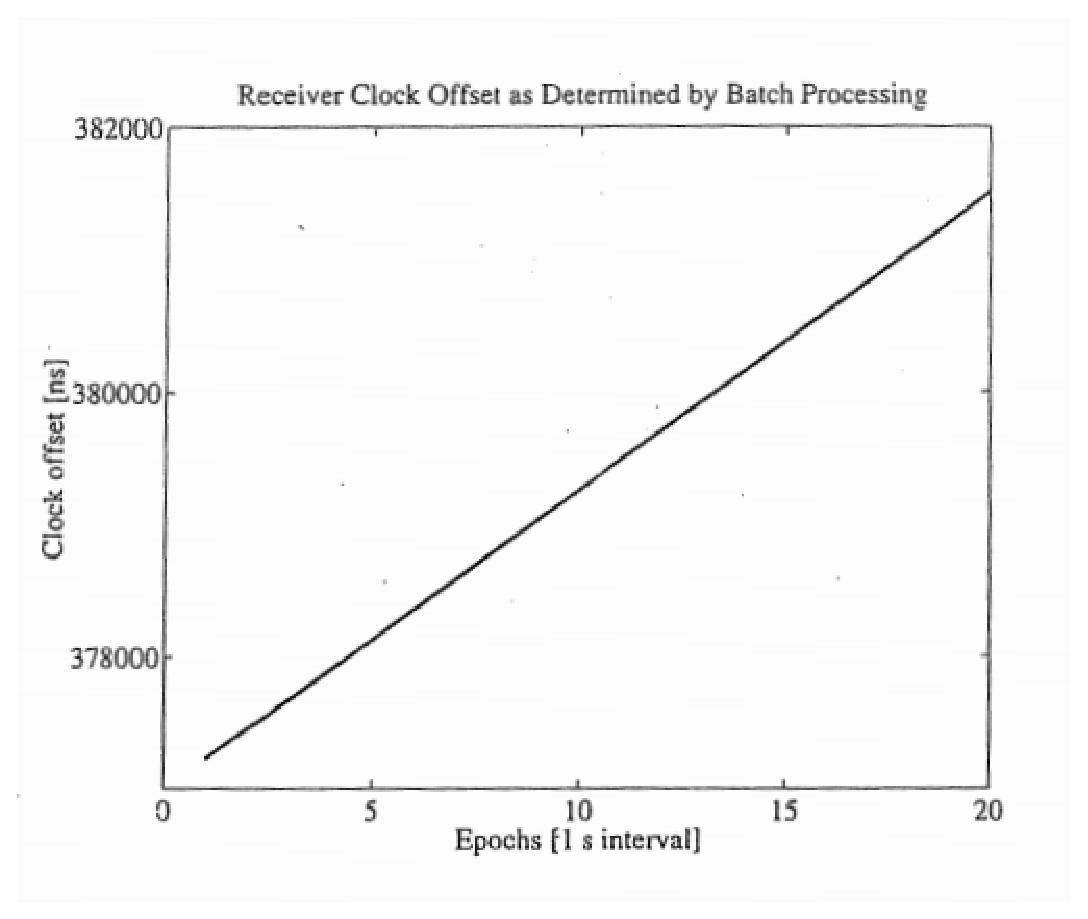
\includegraphics[width=0.7\linewidth]{TeX_files/Part03/chapter09/image/9-6}
		\caption{Receiver}
		\label{fig:9-6}
	\end{figure}

	The X-axis points towards the intersection between Equator and Greenwich meridian. The Z-axis coincides with the spin axis of the Earth. The Z-axis is orthogonal to these two directions and forms a right-handed coordinate system.
	
	The orbit plane intersects the Equator plane in the nodal line. The nodal line has two points in common with the Equator. The point at which the satellite moves from south to north is called the ascending node K. The angle between the Equator plane and the orbit plane is the inclination i. The angle at the Earth’s center C between the X-axis and the ascending node K is called $\Omega$; it is a right ascension. The orbital location closest tothe center of the Earth (at one of the focal point of the orbital ellipse) is called perigee.The angle at C between K and the perigee P is called argument of perigee co\ it increases counter-clockwise viewed from the positive Z-axis.
	\begin{figure}
		\centering
		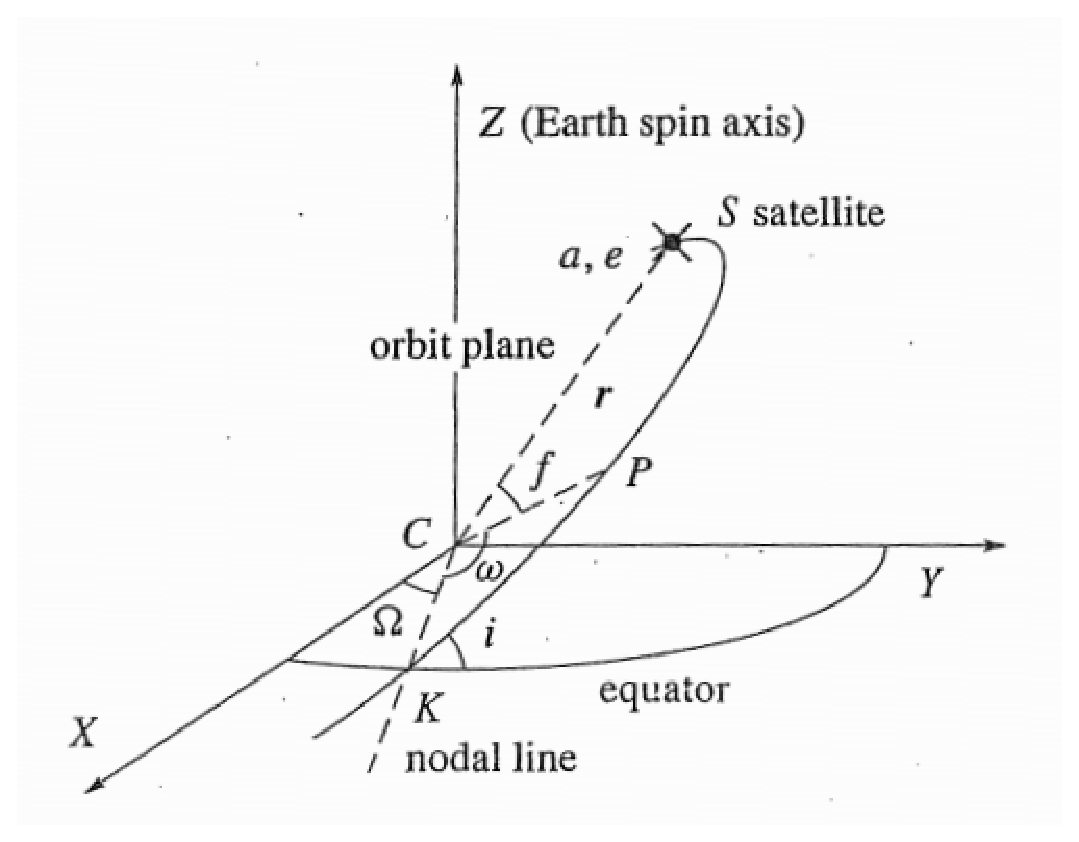
\includegraphics[width=0.7\linewidth]{TeX_files/Part03/chapter09/image/9-7}
		\caption{The Keplerian orbit elements: semi major axis $a$, eccentricity $e$, inclination of orbit $i$ , right ascension $\Omega$ of ascending node $K$ , argument of perigee $\omega$, and true anomaly $f$. Perigee is denoted $P$. The center of the Earth is denoted $C$.}
		\label{fig:9-7}
	\end{figure}

	Figure \ref{fig:9-8} shows a coordinate system in the orbital plane with origin at the Earth’s center C. The $\xi-axis$ points to the perigee and the $\eta-axis$ towards the descending node. The $\xi-axis$ is perpendicular to the orbitplane. From Figure \ref{fig:9-8} we read the eccentric anomaly $E$ and the true anomaly $f$. Also immediately we have
	\begin{figure}
		\centering
		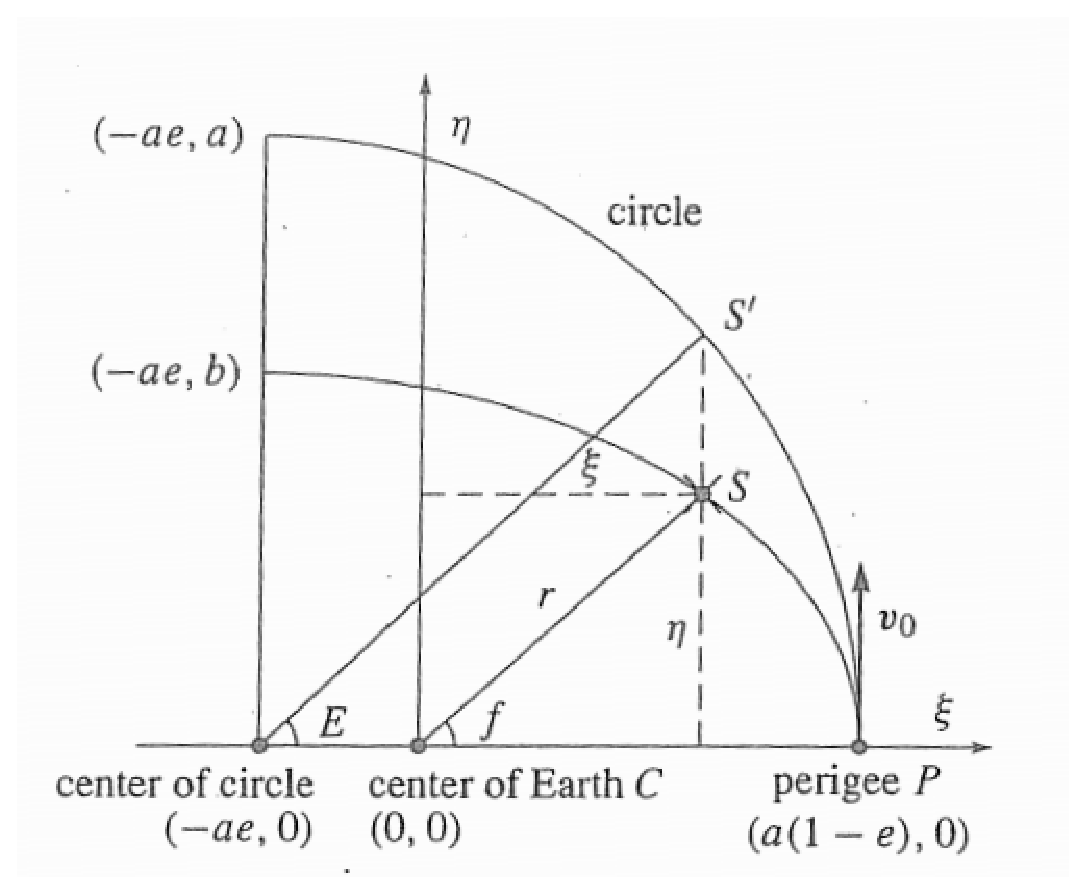
\includegraphics[width=0.7\linewidth]{TeX_files/Part03/chapter09/image/9-8}
		\caption{The elliptic orbit with $(\xi,\eta)$ coordinates. The true anomaly $f$ at $C$.}
		\label{fig:9-8}
	\end{figure}
	$$\xi = r \cos f = a \cos E - ae = a (\cos E -e). $$
	$$\eta = r \sin f = \frac{b}{a} \sin E = b \sin E = a\sqrt{1-e^2}\sin E.$$

	Hence the position vector $r$ of the satellite with respect to the center of the Earth $C$ is
	\begin{equation}\label{eq:9.5}
		r=\begin{bmatrix}
		\xi \\ \eta \\ \zeta
		\end{bmatrix}
		=\begin{bmatrix}
		a(\cos E -e) \\
		a\sqrt{1-e^2}\sin E \\
		0
		\end{bmatrix}.
	\end{equation}
	
	Simple trigonometry leads to the following expression for the norm
	\begin{equation}\label{eq:9.6}
		\lVert r \lVert = a(1-e\cos E).
	\end{equation}
	
	Ingeneral the angle E varies with time t while a and e are nearly constant. (There are long and short periodic perturbations to e, only short for a.) Recall that $\lVert r \lVert$ is the geometric distance between satellite S and the Earth center C = (0, 0, 0).
	
	For later reference we introduce the mean motion n which is the mean angular satellite velocity. If the period of one revolution of the satellite is T , and $GM = 3.986005 • 10^14 m^3/s^2$ we have
	\begin{equation}\label{eq:9.7}
		n = \dfrac{2\pi}{T} = \sqrt{\dfrac{GM}{a^3}}.
	\end{equation}
	It is now time to define mean anomaly $\mu$. It is a non-geometrical quantity defined as the angle between the perigee and a fictitious satellite in a circular orbit with the same focus and the same period as the satellite of interest, but moving with a constant speed. The constant speed is the mean motion of the satellite. The actual and the fictitious satellites cross the apogee-perigee lines in phase, and the mean anomaly of the satellite is the true anomaly of the fictitious satellite. The mean anomaly at epoch/ is given by
	$$\mu = n(t-t_0)$$
	
	where to is the time of the perigee crossing. Note that$\mu$ is a linear function of time and for a circular orbit we have $\mu = f + \omega$, see Misra $\&$ Enge (2006).
	
	Kepler’s famous equation relates two angles, the mean anomaly $\mu$ and the eccentric anomaly E:
	\begin{equation}\label{eq:9.8}
		E = \mu + e\sin E
	\end{equation}
	
	From equation\ref{eq:9.5} we finally get
	\begin{equation}\label{eq:9.9}
		f = \arctan \frac{\eta}{\xi} = \arctan \dfrac{\sqrt{1-e^2}\sin E}{\cos E-e}
	\end{equation}
	By this we have connected the true anomaly /, the eccentric anomaly E , and the mean anomaly $\mu$. These relations are basic for every computation of a satellite position.
	
	The six Keplerian orbit elements constitute an important description of the orbit, so they are repeated in schematic form in Table \ref{tab:9.3}.
	
	It is important to realize that the orbital plane remains fairly stable in relation to the geocentric X, 7, Z-system. In other words: seen from space the orbital plane remains fairly fixed in relation to the Equator. The Greenwich meridian plane rotates around the Earth spin axis in accordance with Greenwich apparent sidereal time (GAST), that is with a speed of approximately 24 h/day. A GPS satellite performs two revolutions a day in its orbit having a speed of 3.87 km/s.
	
	In the orbital plane the Cartesian coordinates of satellite k in Figure \ref{fig:9-7} are given as
	$$\begin{bmatrix}
	r^k_j\cos f^k_j \\
	r^k_j\sin f^k_j \\
	0
	\end{bmatrix},$$
	
	where $r^k_j = \lVert r(t_j)\lVert$comes from (9.6) with a , e , and E evaluated for $t = t_j$.
	
	This vector is rotated into the X,Y,Z coordinate system by the sequence of 3-d .
	rotations in Figure \ref{fig:9-7}:
	$$R_3(-\Omega^k_j)R_1(-i^k_j)R_3(-\omega ^k_j).$$
	
	The matrix that rotates the XY plane by $\varphi$, and leaves the Z direction alone, is
	\begin{equation}\label{eq:9.10}
		R_3(\varphi) = 
		\begin{bmatrix}
			\cos \varphi & \sin \varphi & 0 \\
			-\sin \varphi & \cos \varphi & 0 \\
			0 & 0 & 1
		\end{bmatrix}
	\end{equation}
	
	Similarly $R_1(\varphi)$ gives a rotation about the X-axis:
	
	\begin{table}
		\caption{Keplerian orbit elemetns:Satellite position}
		\label{tab:9.3}
		\begin{tabularx}{\textwidth}{lX}
			\hline $a$ semi major axis &  \multirow{2}*{size and shape of orbit} \\
				   $e$ eccentricity &  \\ 
			\hline $\omega$ argument of perigee & \multirow{3}{150pt}{the orbital plane in the apparent system} \\ 
				   $\Omega$ right ascension of ascending node &  \\ 
				   $i$ inclination &  \\ 
			\hline $\mu$ mean anomaly & position in the plane \\ 
			\hline 
		\end{tabularx} 
	\end{table}
	
	\begin{equation}
		R_1(\varphi) = 
		\begin{bmatrix}
			1 & 0 & 0 \\
			0 & \cos \varphi & \sin \varphi \\
			0 & -\sin \varphi & \cos \varphi \\
		\end{bmatrix}
	\end{equation}
	
	Finally the geocentric coordinates of satellite k at time $t_j$ ; are given as
	\begin{equation}
		\begin{bmatrix}
			X^k(t_j) \\ Y^k(t_j) \\ Z^k(t_j) 
		\end{bmatrix}
		=
		R_3(-\Omega ^k_j)R_1(-i^k_j)R_3(-\omega ^k_j)
		\begin{bmatrix}
			r^k_j \cos f^k_j \\
			r^k_j \sin f^k_j \\
			0
		\end{bmatrix}
	\end{equation}
		
	However, GPS satellites do not follow the presented normal orbit theory. We have to use time dependent, more accurate orbit values: Time-varying Kepler elements or their equivalent. They come to us as the socalled broadcast ephemerides, see below. We insert those values in a procedure given below and finally we get a set of variables to be inserted into (9.12).
	\begin{figure}
		\centering
		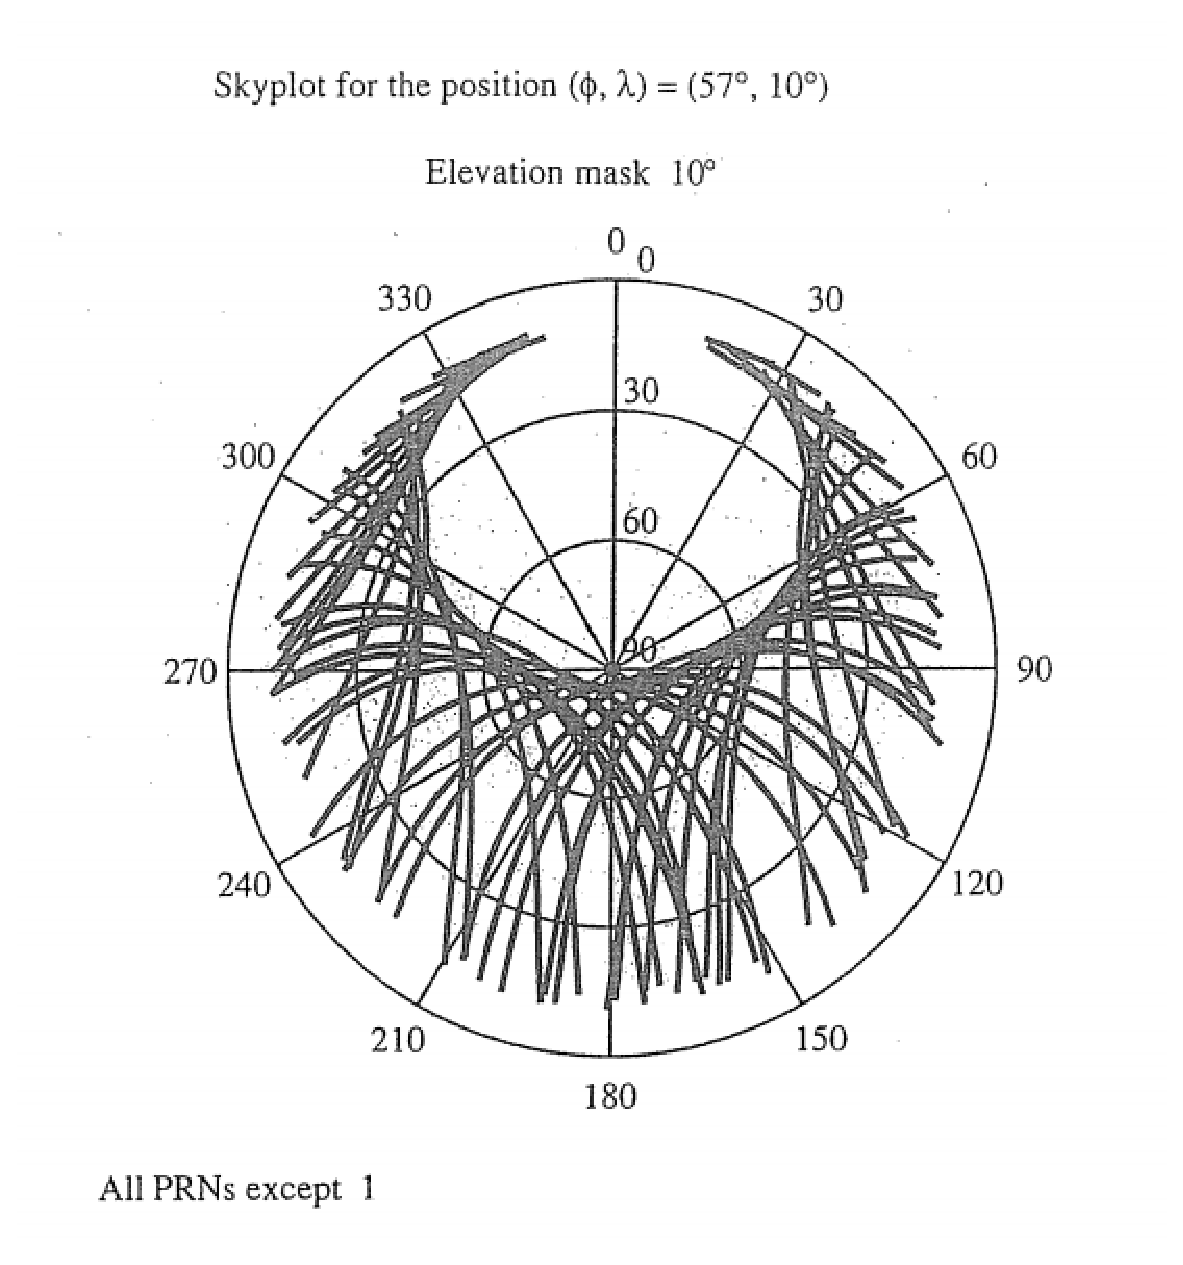
\includegraphics[width=0.7\linewidth]{TeX_files/Part03/chapter09/image/9-9}
		\caption{Skyplot including all GPS satellites for a period of 24 hours at a given position. The elevation mask is $10^\circ$. All PRNs except PRN 1 are plotted.}
		\label{fig:9-9}
	\end{figure}
	
	One speaks about the ephemeris (plural: ephemerides, accent on “ phem” ) of the satellite. These are the parameter values at a specific time. Each satellite transmits its unique ephemeris data. The parameters chosen for description of the actual orbit of a GPS satellite and its perturbations are similar to the Keplerian orbital elements. The broadcast ephemerides are calculated using the immediate previous part of the orbit and they predict the next part of the orbit. The broadcast ephemerides are accurate to 1-2 m. For some geodetic applications better accuracy is needed. One possibility is to obtain post processed precise ephemerides which are accurate at dm-level.
		
	An ephemeris is intended for use from the epoch toe of reference counted in seconds of GPS week. It is nominally at the center of the interval over which the ephemeris is useful. The broadcast ephemerides are intended for use during this period. However they describe the orbit to within the specified accuracy for 2 hours afterward. They are predicted by curve fit to 4-6 hours data. The broadcast ephemerides include
	$$\mu_0,\Delta n,e,\sqrt{a},\Omega_0,i_0,\omega,\dot{\Omega},\dot{i},C_{\omega c},C_{\omega s},C_{rs},C_{ic},C_{is},t_{oe}$$
		
	where $\dot{\Omega}=\partial \Omega / \partial t$and$\dot{i}=\partial i / \partial t$. The coefficients $C_\omega$,$C_r$,and $C_i$; correct argument of perigee, orbit radius, and orbit inclination due to inevitable perturbations of the theoretical orbit caused by variations in the Earth’s gravity field, albedo and sun pressure, and attraction from sun and moon. The reference time of ephemerides parameters is toe. 
		
	Given the transmit time t (in GPST) the following procedure gives the necessary variables to use in (9.12):
	\begin{table}
		\begin{tabularx}{\textwidth}{XX}
			\hline Time elapsed since $t_oe$  & $t_j=t-t_{oe}$ \\ 
				   Mean anomaly at time $t_j$ & $\mu_j = \mu_0 + (\sqrt{GM/a^3}+\Delta n)t_j$ \\ 
   Gravitational constant x mass of the Earth & $GM=3.986005\cdot 10^{14}M^3/S^2$ \\ 
				Iterative solution for $E_j$  & $E_j=\mu_j+e\sin E_j$ \\ 
								True anomaly  & $f_j=\arctan \dfrac{\sqrt{1-e^2}\sin E_j}{\cos E_j-e}$ \\ 
				Longitude for ascending node  & $\Omega_j=\Omega_0 + (\dot{\Omega_0}-\omega_e)t_j-\omega_et_{oe}$ \\ 
						 Mean Earth rotation  & $\omega_e=7.292115147\cdot10^{-5}rad/s$ \\ 
						 Argument of perigee  & $\omega_j=\omega+f_j+C_{\omega c}\cos2(\omega+f_j)+C_{\omega s}\sin2(w+f_j)$ \\ 
							 Radial distance  & $r_j = a(1-e\cos E_j)+C_{rc}\cos 2(\omega+f_j)+C_{rs}\sin 2(\omega+f_j)$ \\ 
								 Inclination  & $i_j = i_0+\dot{i}t_j+C_{ic}\cos 2(\omega+f_j)+C_{is}\sin 2(\omega+f_j)$ \\ 
			\hline 
		\end{tabularx} 
	\end{table}
		
	The algorithm that computes (9.12) is coded as the M -iile satpos. The function calculates the position of any GPS satellite at any time. It is fundamental to every position calculation. For more details on the WGS 84 in connection with GPS, see Section 3.6.
		
	The M-file satposin computes satellite positions in an inertial frame where $\omega_e$ = 0.
		
	All information about the Kepler elements is contained in the ephemerides. Files containing broadcast ephemerides are created when downloading the GPS observations to a laptop. These files most often are in a receiver specific binary format. Fortunately these formats can be converted into the RINEX format, see Gurtner (2000). The third character in the extension of such files is always n (for navigation).
		
	Often we only need part of the information in the navigation file for the ephemeris file. The selection and reformatting is done via the following commands:
	\begin{lstlisting}
		rinexe(ephemerisfile,outputfile);
		eph=get_eph(outputfile);
		satp=satpos(t,eph);
	\end{lstlisting}
	\subsection{easy2}\label{subsec:easy2}
		The second basic issue is to compute the position in the Earth Centered Inertial frame (ECI) of a given pseudo random noise satellite at a given time. The ECI coordinate system for GPS uses the orientation of the Earth equatorial plane at 12 hours UTC on January 1,2000. The X-axis points to the vernal equinox, the Z-axis points in the direction of the North Pole, and the Y -axis is chosen as to form a right-handed coordinate system.
		\begin{figure}
			\centering
			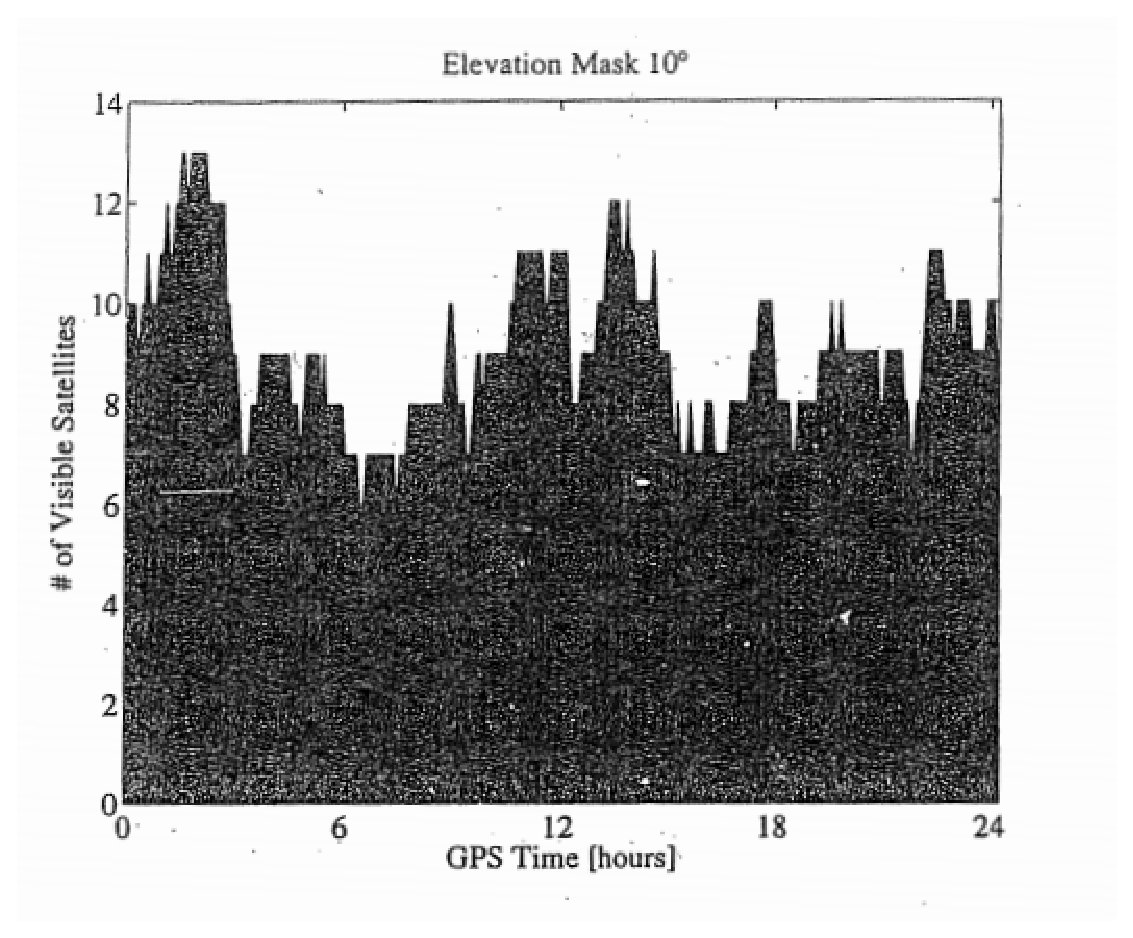
\includegraphics[width=0.7\linewidth]{TeX_files/Part03/chapter09/image/9-10}
			\caption{Number of satellites $10^\circ$ or higher above the horizon}
			\label{fig:9-10}
		\end{figure}
	
		Given an ephemeris obtained from a RINEX Navigation Message file (n-file), easy2 does the job. The main function satpos implements the procedure described in the GPS Interface Control Document (IS-GPS-200 (2007)), Table 20-IV.
		
		We read a RINEX n-file and reformat it into MATLAB’s internal format as a matrix named Eph. Furthermore, we relate each PRN to a column of Eph. Each column contains 21 variables; these comprise a complete ephemeris for one satellite.
	
	\subsection{easy11}\label{subsec:easy11}
		Figure \ref{fig:9-9} shows a polar plot of satellite orbits as viewed from a given location on Earth.You can see the period of time when each satellite is visible during 24 consecutive hours.
		\begin{figure}
			\centering
			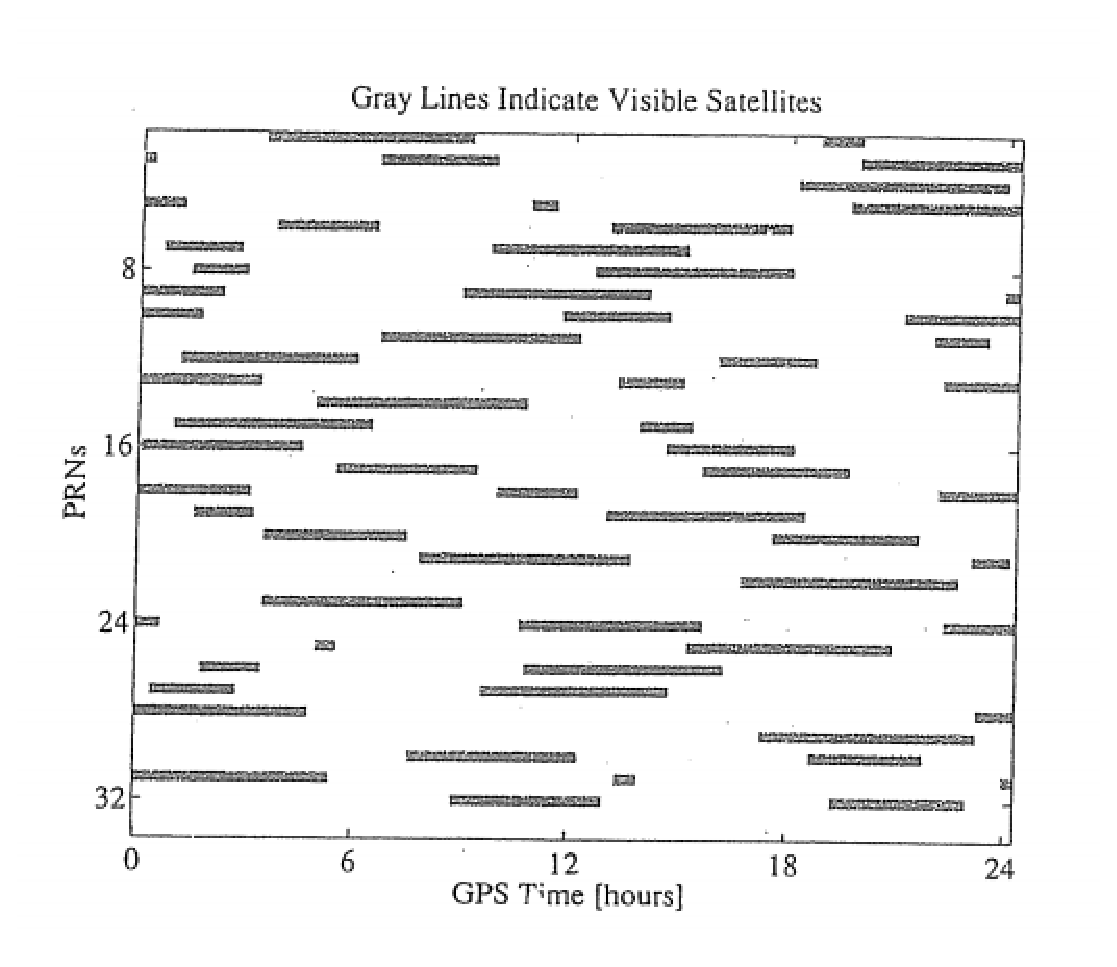
\includegraphics[width=0.7\linewidth]{TeX_files/Part03/chapter09/image/9-11}
			\caption{Time period when the visible satellites are $10^\circ$ or higher above the horizon at position $\varphi = 57^\circ$ and $\lambda = 10^\circ$}
			\label{fig:9-11}
		\end{figure}
		
		easyl 1 is based on an almanac downloaded most easily from the National Geodetic Survey at ngs.noaa.gov/CORS/Data.html. The actual file name is brdcl 550.08n.
		
		The RINEX file has been reformatted into MATLAB’s binary format for satellite ephemerides using the A/-file rinexe. The user enters $(\varphi,\lambda)$ for the position on the ground where the plot is to be used, and a value for the levation mask to be set. Then the azimuth and elevation angles for all visible positions of the included satellites are computed and plotted as polar coordinates.
		
		Next follows bookkeeping on how many and which satellites are visible during the day and the time periods when they can be seen. Figures \ref{fig:9-10} and \ref{fig:9-11} show the plots.
		
		The MATLAB code is simple, the result is impressive, and it is useful. In early GPS days when the constellation was incomplete, such plots were especially valuable for planning purposes to be sure that enough satellites would be available for positioning.Except in the most severe terrain and urban canyons, receivers can find plenty of GPS	(and GLONASS) satellites around the clock, and this situation will become even more satisfactory when Galileo satellites are launched.
	

	
	
